% --- Program Section ---

\newprogram{Program 16}{ Implement strStr(haystack: str, needle: str) -> int using KMP and a Randomizer class with
getRandom() -> int for stream sampling, accepting text/pattern strings or stream data and returning
indices or sampled elements.}
\subsection*{Code}


\begin{lstlisting}[language=python]
from typing import Iterator, Optional
import random

# KMP String Matching
def strStr(haystack: str, needle: str) -> int:
    if needle == "":
        return 0

    # Build LPS (Longest Prefix Suffix) array
    lps = [0] * len(needle)

    length = 0
    i = 1

    while i < len(needle):
        if needle[i] == needle[length]:
            length += 1
            lps[i] = length
            i += 1
        elif length > 0:
            length = lps[length - 1]
        else:
            lps[i] = 0
            i += 1

    # Search needle inside haystack
    i = 0
    j = 0

    while i < len(haystack):
        if haystack[i] == needle[j]:
            i += 1
            j += 1

            if j == len(needle):
                return i - j

        elif j > 0:
            j = lps[j - 1]
        else:
            i += 1

    return -1
# Reservoir Sampling
class Randomizer:

    def __init__(self, stream):
        self.stream = stream
        self.selected = None

    def getRandom(self) -> int:
        """
        Return one uniformly random element from the stream.
        """

        selected = None

        for i, value in enumerate(self.stream, start=1):

            # Replace selected element with probability 1/i
            if random.randint(1, i) == 1:
                selected = value

        return selected
# Examples
print("KMP result:")
print(strStr("hello", "ll"))

print("\nRandom stream sample:")

stream = [10, 20, 30, 40, 50]

randomizer = Randomizer(stream)

print(randomizer.getRandom())
\end{lstlisting}

\subsection*{Output}
\begin{center}
    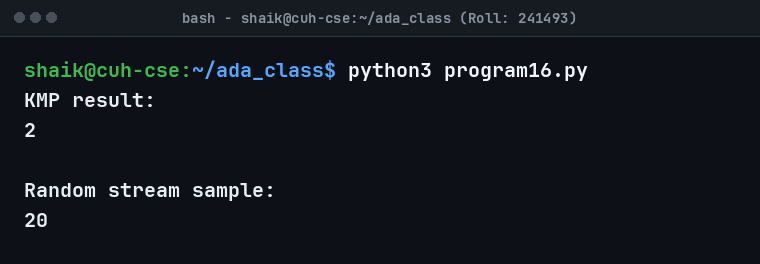
\includegraphics[width=0.88\textwidth]{Images/output_screenshot16.png}
\end{center}

\subsection*{GitHub Scan Code}
\begin{center}
    \begin{minipage}{0.3\textwidth}
        \centering
        % Generates a 2.5cm high QR code directly linking to the code file
        \qrcode[height=3.5cm]{https://github.com/gytdrop/ada_class/blob/main/program16.py} \\[0.2cm]
        \scriptsize\ttfamily Scan to view source code 
    \end{minipage}
\end{center}


% Add a horizontal line that indicates the END of the program.
\vspace{1cm}
\begin{center}
    \rule{1\textwidth}{1pt} % Clean, centered 1pt thick horizontal line
\end{center}